%! TEX root = ../main.tex

\chapter{The Pierre Auger Observatory}
\label{chap:pierre-auger-observatory}

The \PAO is the (by area) largest scientific experiment in the world. It 
consists of an array of 1660 \WCDs, which form the \SD, and 27 fluorescence 
telescopes, that make up the \FD.

With a region spanning roughly \SI{3000}{\kilo\meter\squared} it offers a unique
possibility to observe \UHECRs at the tail-end of the \CR energy spectrum with
an unprecedented accuracy and precision.

We begin this chapter in \cref{sec:science-case} by formulating open questions 
that the \PAO aims to answer. Design details for the \FD and for the \SD are 
given in \cref{sec:fd} and \cref{sec:sd} respectively. After a discussion on the
local \DAQ process and the centralized event detection in \cref{sec:cdas}, we 
finish by detailing the procedure of the event reconstruction and higher level 
analysis in \cref{sec:rec}.

\section{Science Goal and Open Questions}
\label{sec:science-case}

The flux of cosmic rays with energies exceeding the ankle, $\SI{5e18}{\eV}$, is 
very low, and measures on average 6 events per \SI{}{\km\squared\year}
\cite{Fenu2023}. It is evident that one needs a large detector and a lot of time
in order to make statistically relevant statements about the physics of \UHECRs.
Altough only one of the initially planned two data taking sites came to reality 
\cite[for white paper see][]{Zavrtanik2000}, the Pierre Auger observatory has 
been be a world-leading experiment in terms of measured exposure from the 
beginning of \DAQ in January 2004 \cite{Abraham2004}, and will continue to yiel
results until decomission after 2030 \cite{Castellina2023}.

Many insights, such as the existence of the \CR dipole discussed in
\cref{sec:cr-origins}, have been gathered from Augers event database as a 
consequence. Still, a plethora of mysteries remain. It follows a list of, in no 
particular order, important missing links of information that motivate not least
this thesis, but the continued effort and daily work done by the Auger 
collaboration.

\subsection{Flux supression at highest energies}
\label{ssec}

\subsection{Validity of shower simulations}


\subsection{Exotic events}
\subsubsection{Photon showers}
\subsubsection{Neutrino showers}
\subsubsection{GZ effect}

\section{The Fluorescence Detector}
\label{sec:fd}

The Fluorescence Detector of the \PAO is a set of 27 reflector telescopes tuned
to detect faint sources of \UV light. More specifically, the aim of the \FD is
to observe \UV-emission of \EAS. However, since the solar irradiance 
(\SI{120}{\watt\per\meter\squared} @
\SIrange[range-phrase={--}]{200}{400}{\nano\meter} \cite{Snow2013}) and even the
lunar irradiance (\SI{16}{\nano\watt\per\meter\squared} @
\SIrange[range-phrase={--}]{180}{300}{\nano\meter} \cite{Lean1989}) in the 
\UV-band far outshine the emission of \UV-light by cosmic rays 
(\SI{0.32}{\nano\watt\per\meter\squared} @ \SI{337}{\nano\meter} 
\cref{app:cr-uv-irradiance}), the \FD can only operate in the astronomical night
during third to first quarter moon. This consequently drops the duty cycle to 
approximately 20\%\todo{cite}.

\subsection{Telescope and camera design}
\label{ssec:fd-design}

\subsection{Calibration of measurements}
\label{ssec:fd-calibration}

\subsubsection{Drum calibration}
\subsubsection{XY-scanner}

\section{The Surface Detector}
\label{sec:sd}

\todo[inline]{roughly mention design, duty cycle}

\section{Central Data Acquisition System}
\label{sec:cdas}



\section{\Offline and Event Reconstruction}
\label{sec:rec}

\begin{figure}[t]
  \centering
  \subfloat[]{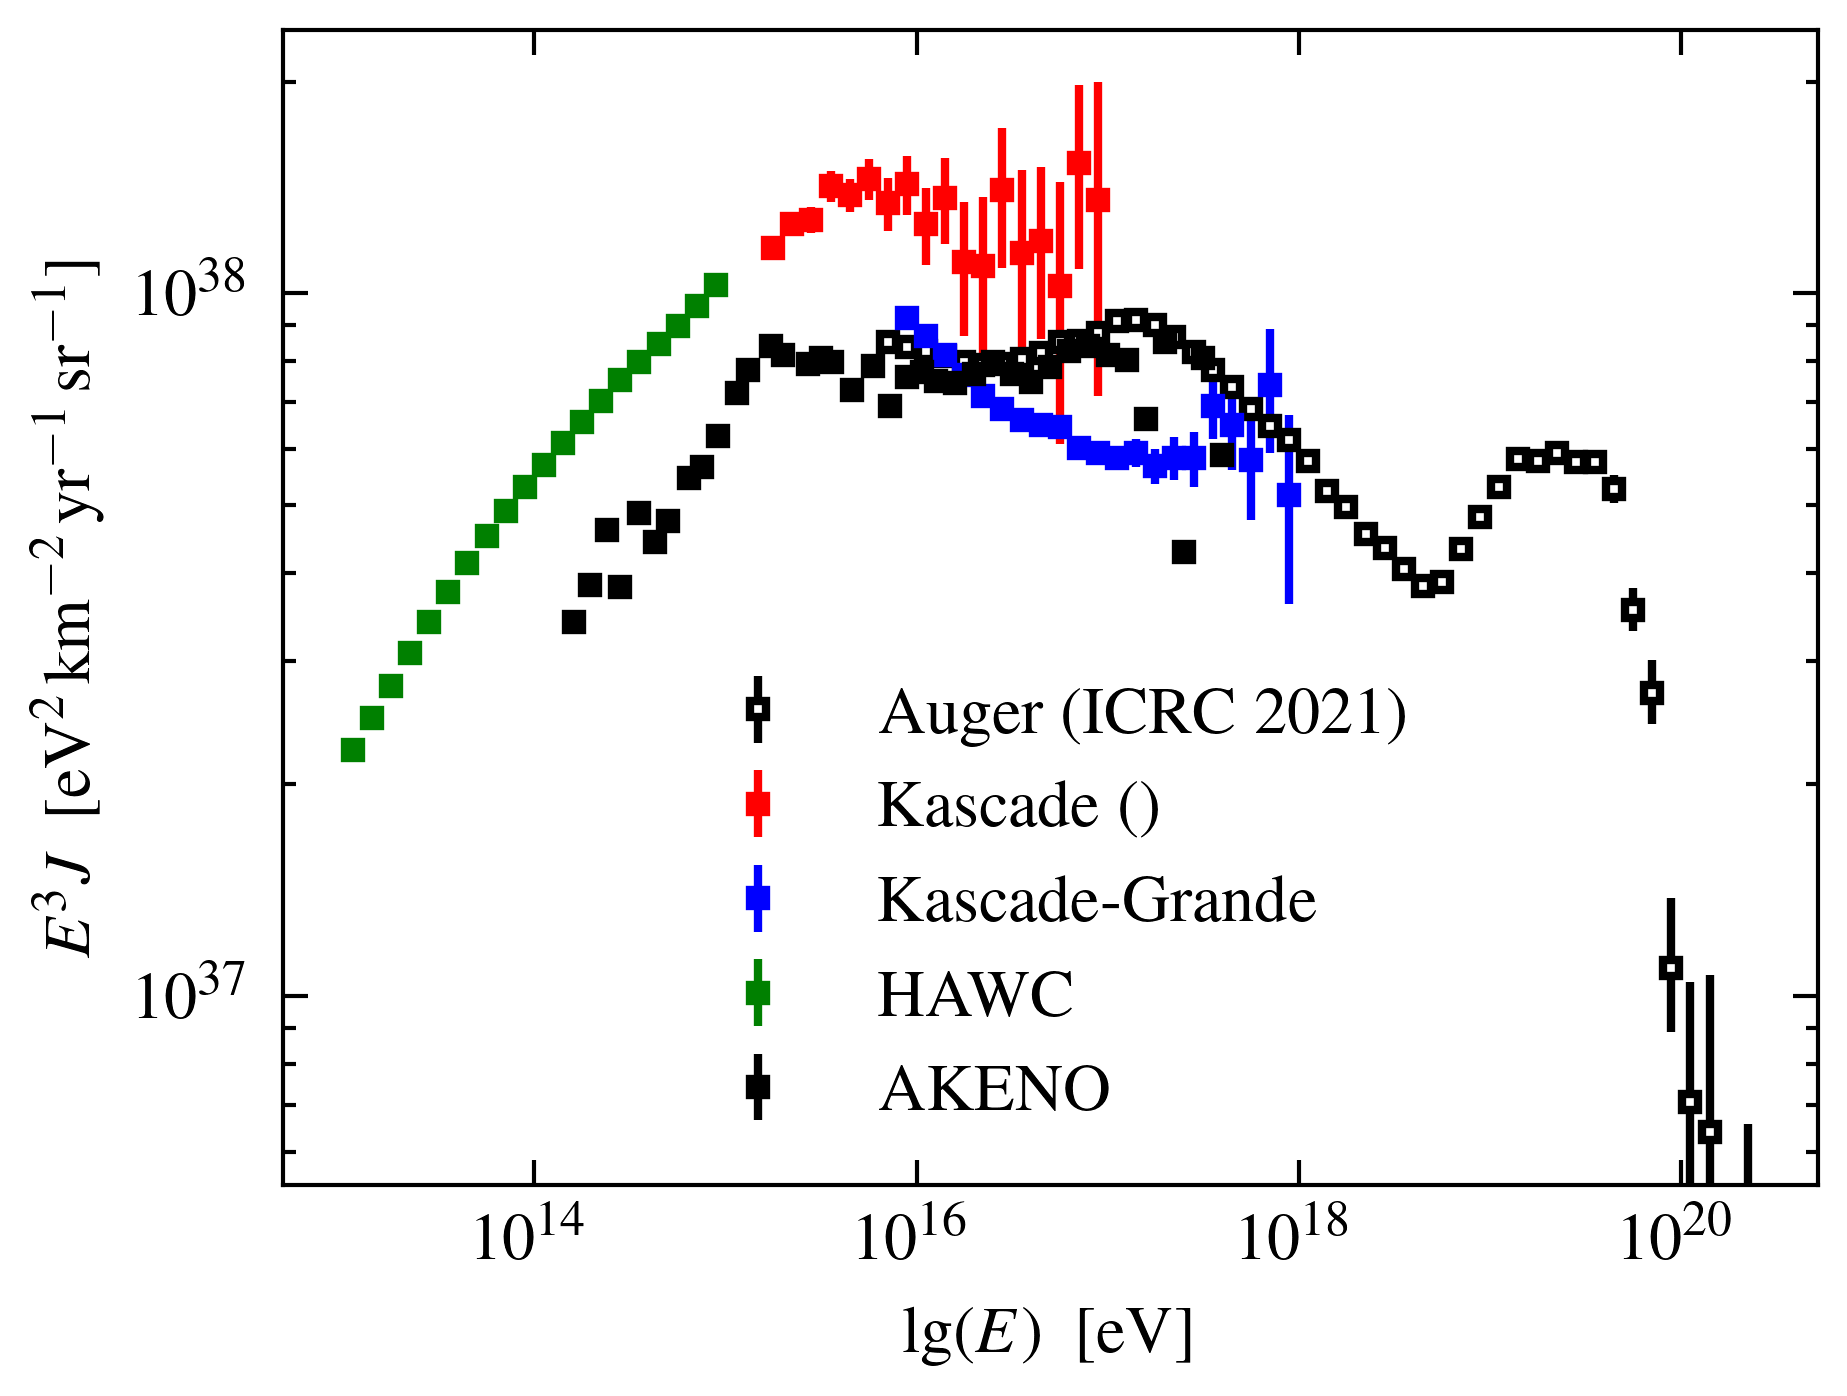
\includegraphics[width=0.47\textwidth]{cosmic-rays/spectrum-double1.png}
  \label{fig:LABEL}
  }\hspace{0.2cm}
  \subfloat[]{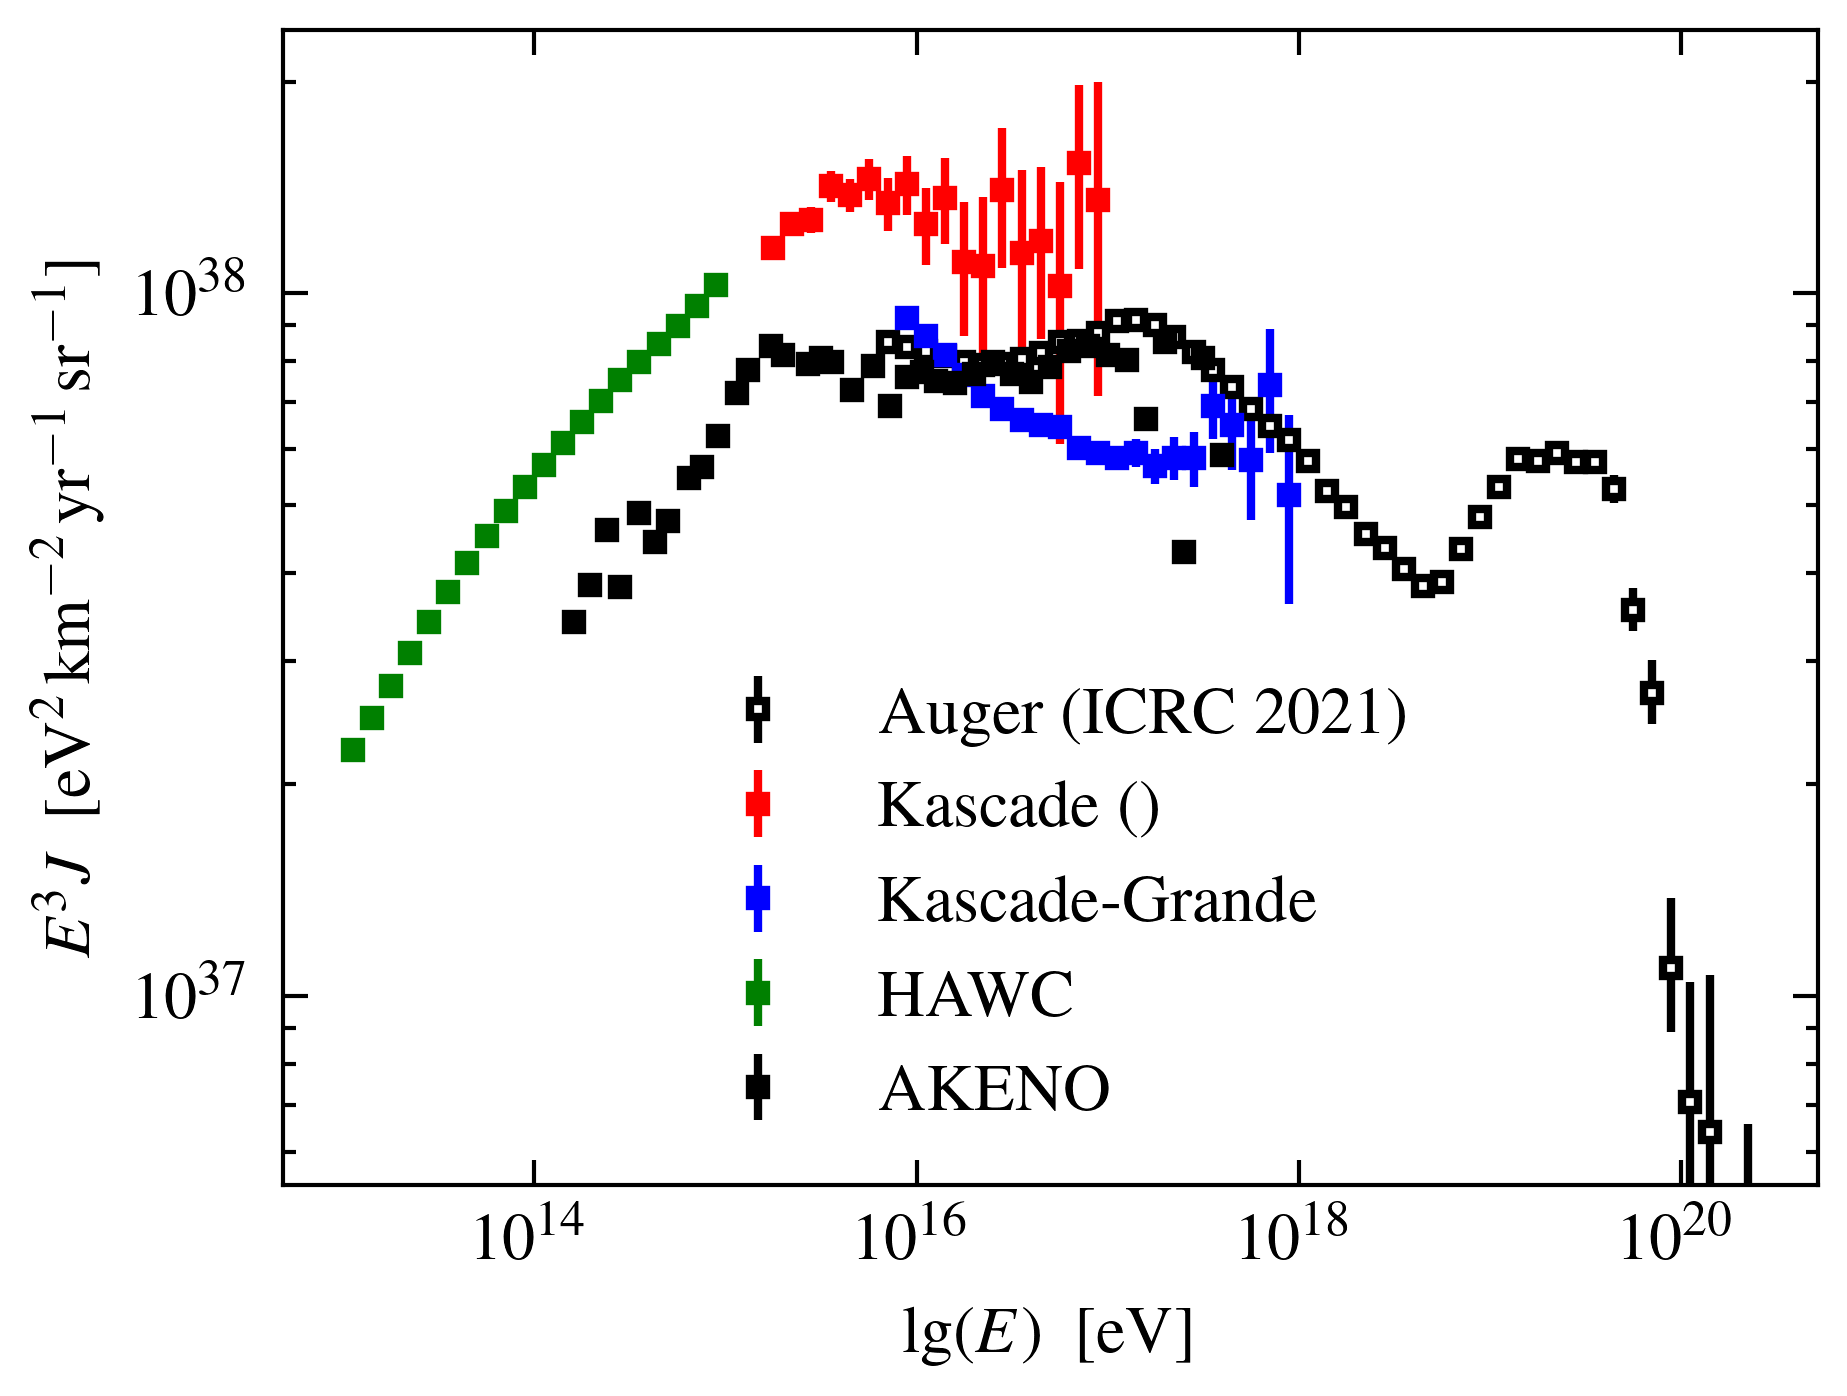
\includegraphics[width=0.47\textwidth]{cosmic-rays/spectrum-double2.png}
  \label{fig:LABEL}
  }
  \caption[]{\subref{fig:LABEL} asdasd \subref{fig:LABEL} asdasd}
  \label{fig:}
\end{figure}

\begin{figure}[t]
  \centering
  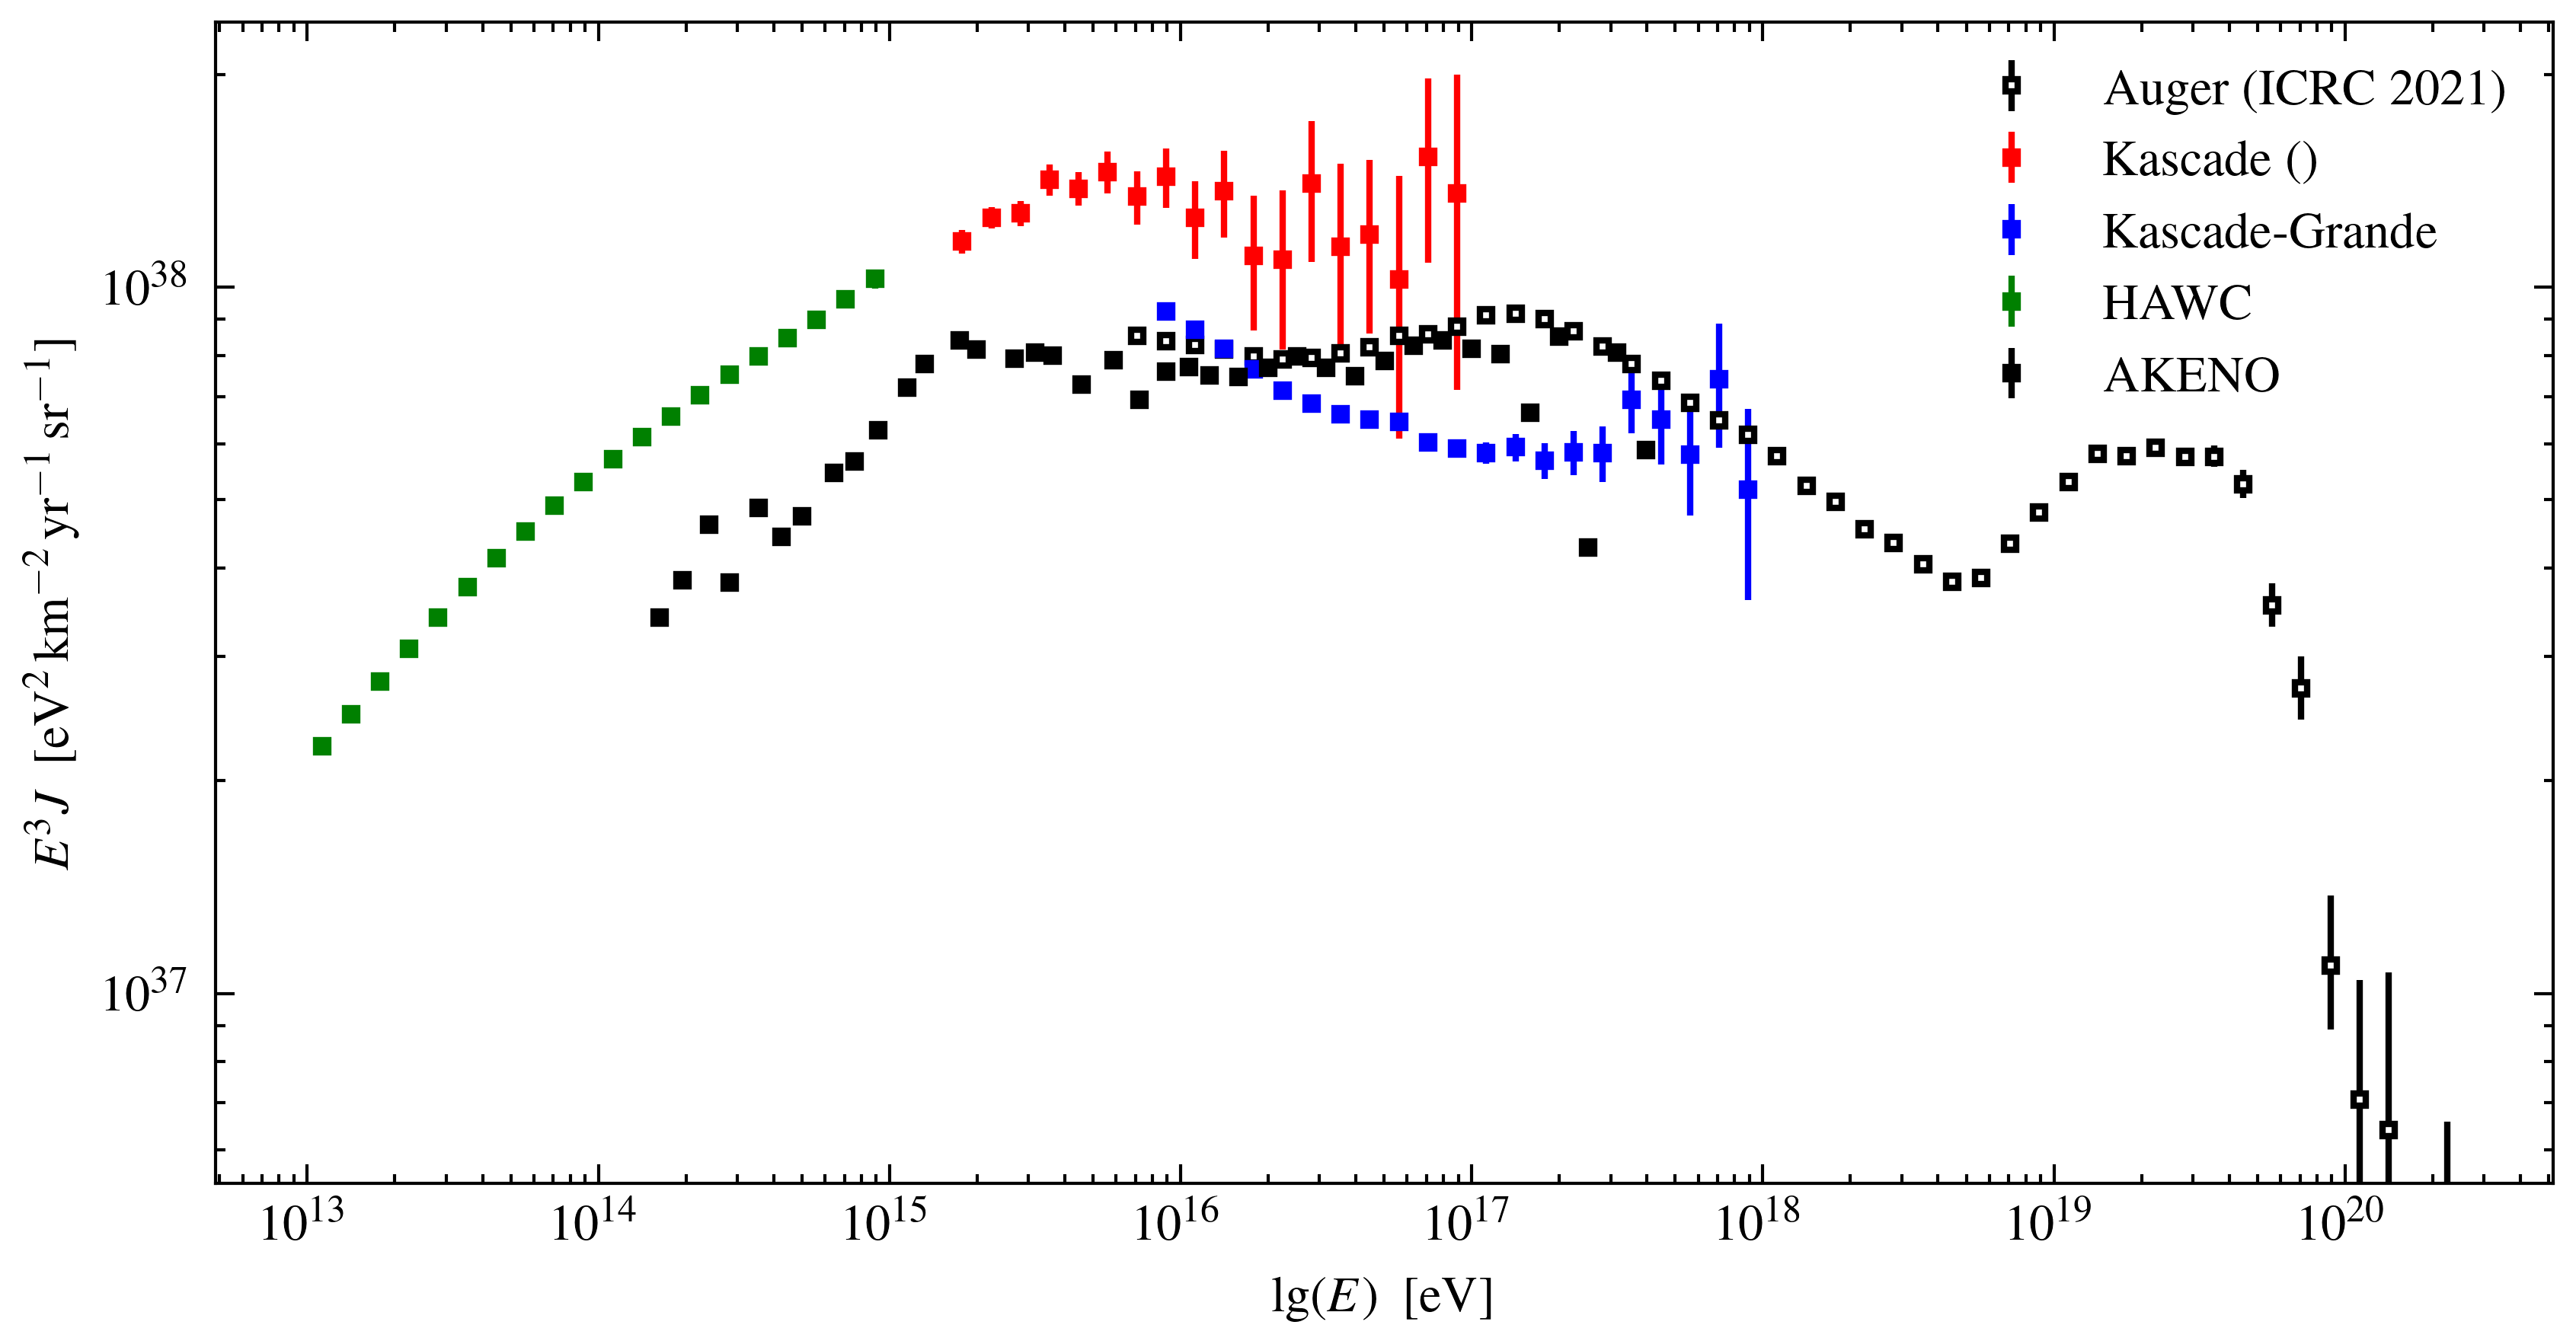
\includegraphics[width=0.9\textwidth]{cosmic-rays/spectrum-single.png}
  \caption{asdasdasdasd}
  \label{fig:asdasd}
\end{figure}


